\documentclass{homework}
\usepackage[utf8]{inputenc}
\usepackage{xspace,color,url,listings,graphicx,float,amsmath,amssymb,braket,subcaption}
\graphicspath{{./graphs/}} %location of images

\lstset{commentstyle=\color{red},keywordstyle=\color{black},
showstringspaces=false}
\lstnewenvironment{py}[1][]{\lstset{language=Python}}{}
\newcommand{\pyt}[1]{\lstinline{#1}}  %% Short for 'Python inline'

\lstset{language=Python}             % Set Py to default language

\newcommand{\hwname}{Shara Duong, Charles Colgan, Josh Borders}
\newcommand{\hwnum}{3}

\newcommand{\hwtype}{Homework}
\newcommand{\hwclass}{MATH 6373}

\begin{document}

\maketitle

Shara Duong: Wrote code\\
Charles Colgan: Edited report. \\
Josh Borders: Wrote report. \\

\question*{Introduction and Data Description}
The goal of this homework is to implement a convolution neural network (CNN) in order to classify images of different fonts. Our data has five font classes - Bistream Vera, Consolas, Century, Ebrima, and Gill - with 9762 total cases, where each case is an image of a character belonging to one of the fonts. The composition of our data is displayed in Table \ref{case_comp}.

\begin{table}[h]
    \centering
    {\begin{tabular}{c|cc|c}
         &Training&Testing&Total\\
         \hline
         Bitstream&1837&459&2296\\
         Consolas&1828&457&2285\\
         Century&1599&400&1999\\
         Ebrima&1379&344&1723\\
         Gill&1167&292&1459\\
         \hline
         Total&7810&1952&\textbf{9762}
    \end{tabular}}\\
    \caption{Number of Cases for Each Class}
    \label{case_comp}
\end{table}

\question*{Reshaping the Input Data}
The input data is in the form of a flattened vector of length 400, with each feature being the intensity of black in a corresponding pixel, on a scale of 0 to 255. We standardized these values so that values they are constrained between 0 and 1. Reshapeing these vectors into 20x20 matrices, results in the original images. We used Numpy's reshape function to convert our 9762 vectors into  appropriate matrix form.\\\\
Figure \ref{image_ex} shows the letter 'p' for each of our five classes. From a cursory glance, Bitstream and Gill appear to have thicker line work covering more pixels than Century and Ebrima, which have line work that covers comparatively fewer pixerls.

\begin{figure}[H]
\begin{subfigure}{0.4\textwidth}
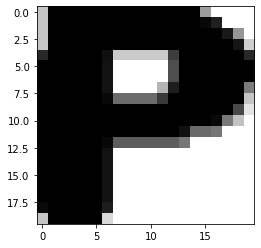
\includegraphics[width=\linewidth]{bit_p.png}
\caption{Bitstream} \label{fig:a}
\end{subfigure}\hspace*{\fill}
\begin{subfigure}{0.4\textwidth}
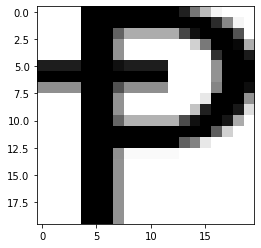
\includegraphics[width=\linewidth]{con_p.png}
\caption{Consolas} \label{fig:b}
\end{subfigure}

\medskip
\begin{subfigure}{0.4\textwidth}
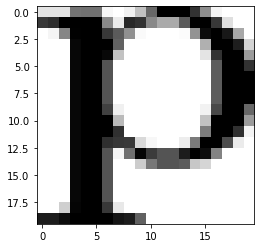
\includegraphics[width=\linewidth]{cent_p.png}
\caption{Century} \label{fig:c}
\end{subfigure}\hspace*{\fill}
\begin{subfigure}{0.4\textwidth}
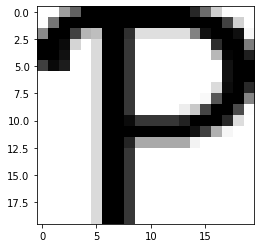
\includegraphics[width=\linewidth]{ebrima_p.png}
\caption{Ebrima} \label{fig:d}
\end{subfigure}


\medskip
\begin{subfigure}{0.4\textwidth}
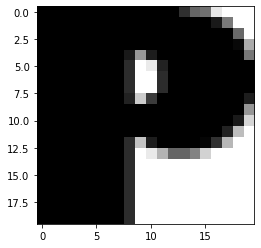
\includegraphics[width=\linewidth]{gill_p.png}
\caption{Gill} \label{fig:e}
\end{subfigure}\hspace*{\fill}
\caption{P in Different Fonts}
\label{image_ex}
\end{figure}

\question*{CNN Architecture}
We now define an architecture for our convolution neural network (CNN). It consists of two instances of convolution followed by max pooling layers, a flattening layer, a dense MLP with hidden layer of size h, and a five-dimension output layer. The activation function for both convolution layers and the MLP is RELU, and the activation function for the output layer is softmax.\\\\
The data is input as a 20x20 image and is fed to the first convolution layer. Here, the image is processed by taking a 5x5 window and viewing across the image with a stride of 1. The pixels indexed by the center of the window are kept and the input image is thereby reduced to size 16x16. This layers has contains 16 channels and thus 16 images are sent to the next layer. Then going to the first max pool layer, a 2x2 window with stride 2 is employed in a similar fashion to the first convolution layer. The pixels indexed by the window are treated as a new pixel and thus the 16 images of dimension 16x16 now become 16 images of dimension 8x8. These are passed to another convolution layer with a 3x3 window and processed with a stride of 1. This layer also has 16 channels, resulting in 16 images of size 6x6. Finally, the images are provided to another max pool layer with a 2x2 window and stride 2. The result of this convolution and pooling process is the reduction a single image of size 20x20 to 16 images of size 3x3, with the goal of extracting important features from the data.\\\\
These 16 3x3 images are next flattened into a long vector of dimension 144. This vector becomes the input to a dense MLP with a single hidden layer of size h, which will be selected during training from among the values of 90, 150, and 200.\\\\
The number of parameters, all weights and biases, the network needs to learn and the distribution of these parameters are provided in Table \ref{parameters}. The number of convolution parameters (i.e., the parameters located in all layers preceding the MLP) are fixed at 4674, while the number of MLP parameters depends on the size of h. As h increases, the percentage of parameters belonging to the convolution network decreases.\\\\
The amount of information brought to the network by our training set with 7810 cases is 39,050, or 7810*5. Ideally, the number of parameters learned by the network will be less than the amount of information provided by the training set. This is true for all three of our potential values of h.

\begin{table}[h]
    \centering
    {\begin{tabular}{c|ccc|c}
         h&Convolution&MLP&Total&Percent Convolution\\
         \hline
         90&4674&13505&18179&25.7\%\\
         150&4674&22505&27179&17.2\%\\
         200&4674&30005&34679&13.5\%\\
    \end{tabular}}\\
    \caption{Number of Parameters for Each Potential Network}
    \label{parameters}
\end{table}

\question*{Training the Network}
Training of the CNN was completed in Google Colab. Our training set was of size 7810, and our test set was of size 1952. The batch size was taken the square root of the size of the training set, giving us an approximate batch size of 89. We used the RELU function as our activation function and cross entropy as our loss function. The loss function was minimized using ADAM gradient descent. Dropout learning was utilized at a rate of 50\% for the MLP hidden layer to reduce overfit.\\\\
The computing time for the network for each value of h is provided in Table \ref{computing}. Each training was 100 epochs in length. Doubling the size of the hidden layer only results in a small increase in computing time, so this will likely not be a major factor for selection of the best network.

\begin{table}[h]
    \centering
    {\begin{tabular}{c|c}
         h&Computing Time (seconds)\\
         \hline
         90&232\\
         150&242\\
         200&240\\
    \end{tabular}}\\
    \caption{Computing Time for Each Size of H}
    \label{computing}
\end{table}

\question*{Results and Analysis}
The results of the training are presented in Figure \ref{performance}.\\\\
The first task is to determine where learning should stop, with the goal of avoiding overfit. For h=90, the test loss begins to stabilize around epoch 40, reaching its minimum value at epoch 57, and then begins to slowly trend upward again. While the upward trend is not severe, it is still best to stop learning at the \textbf{57th epoch}. Confusion matrices for h=90 at the stopping time, epoch 57, are provided in Table \ref{confusion}.\\\\
H=150 more clearly shows potential for overfitting the training data, with the test loss stabilizing around the fortieth epoch, and then trending upward at about epoch 60. The minimum test loss is reached in between these values at \textbf{epoch 54}, and it is where learning will stop. Confusion matrices are reported in Table \ref{confusion}.\\\\
H=200 is similar to H=150 in the sense that the potential for overfit is more obvious from the graph. Its testing loss stabilizes at around epoch 30 and starts overfitting around epoch 60, which is very close (0.002) to where the minimum value is reached. Epoch 60 is where learning will stop, and the confusion matrix is reported in Table \ref{confusion}.

\begin{figure}[H]
\begin{subfigure}{0.4\textwidth}
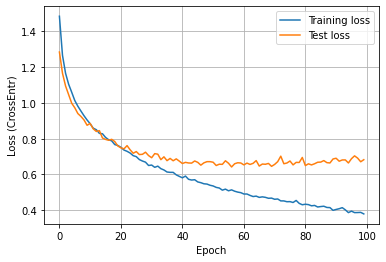
\includegraphics[width=\linewidth]{hw3_h90_loss.png}
\caption{H = 90 Loss Curves} \label{fig:a}
\end{subfigure}\hspace*{\fill}
\begin{subfigure}{0.4\textwidth}
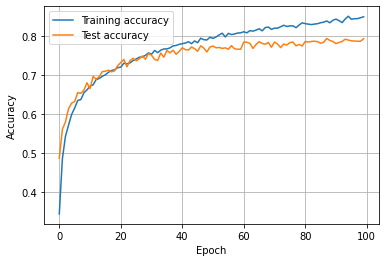
\includegraphics[width=\linewidth]{hw3_h90_acc.png}
\caption{H = 90 Accuracy Curves} \label{fig:b}
\end{subfigure}

\medskip
\begin{subfigure}{0.4\textwidth}
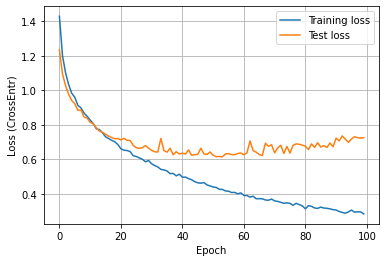
\includegraphics[width=\linewidth]{hw3_h150_loss.png}
\caption{H = 150 Loss Curves} \label{fig:c}
\end{subfigure}\hspace*{\fill}
\begin{subfigure}{0.4\textwidth}
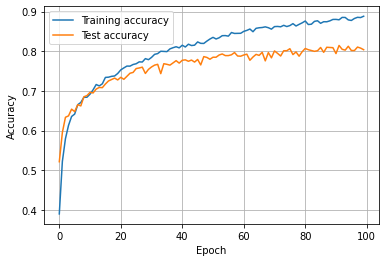
\includegraphics[width=\linewidth]{hw3_h150_acc.png}
\caption{H = 150 Accuracy Curves} \label{fig:d}
\end{subfigure}

\medskip
\begin{subfigure}{0.4\textwidth}
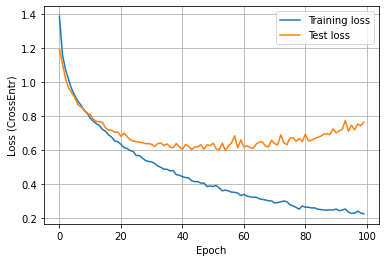
\includegraphics[width=\linewidth]{hw3_h200_loss.png}
\caption{H = 200 Loss Curves} \label{fig:e}
\end{subfigure}\hspace*{\fill}
\begin{subfigure}{0.4\textwidth}
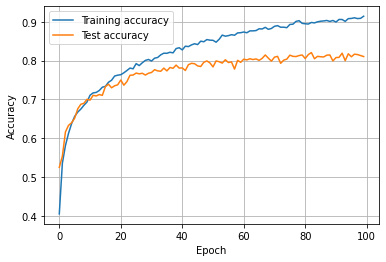
\includegraphics[width=\linewidth]{hw3_h200_acc.png}
\caption{H = 200 Accuracy Curves} \label{fig:f}
\end{subfigure}
\caption{Loss and Accuracy Curves for Each Value of H}
\label{performance}
\end{figure}

Table \ref{confusion} shows confusion matrices for both training and testing sets for each size of h, presented at their respective stopping times. The confusion matrix contains the true class value on the rows and the predicted class value on the columns. Correctly identified entries are logged on the diagonals. As an example, at h=90, Century is mistaken as Bitstream for 0.4\% of training cases (row 2, col 1), while Century is mistaken as Consolas 0.5\% of the time (row 2, col 3). Century is correctly predicted in the training set 87.1\% of the time (row 2, col 2).\\\\
On the whole, the networks do a good job classifying the Bitstream font, often at a rate of 95\% or higher, a decent, unspectacular job of classifying Century and Consolas, and a poor job of classifying Ebrima and Gill. The most striking observation of the confusion matrices, in our opinion, is how the networks regularly underestimate the presence of Ebrima and Gill cases, predicting cases as belonging to them only about three-quarters of the time. The networks thereby overestimate the presence of the former three fonts, which may account for their decent to solid performances. If someone walks into a house blindfolded and is told to correctly guess the color each room is painted, and they guess "brown" for every single room, they'll correctly predict the rooms which are actually brown, while ignoring those that are painted, say, mauve. In the matter of our neural networks, this comparison is not flattering. \\\\
The best performance on both training and testing sets is reached when h is of size 200, with a global accuracy on the training set of 91.4\% and on the testing set of 80.2\%. However, 95\% confidence intervals for global accuracy show slight overlap between the point estimate for this best architecture of h=200 and the others. So, although h=200 has the highest point estimate of global accuracy on both training and testing sets, it is not significantly better than the others in the testing environment. 

\begin{table}[H]
    \centering
    \subfloat[h=90 Training (tstop = 57)]{\begin{tabular}{c|ccccc}
         &BITSTREAM&CENTURY&CONSOLAS&EBRIMA&GILL\\\hline
         BITSTREAM&0.969&0.004&0.018&0.001&0.008\\
         CENTURY&0.004&0.871&0.005&0.048&0.025\\
         CONSOLAS&0.020&0.043&0.869&0.027&0.040\\
         EBRIMA&0.008&0.051&0.144&0.760&0.037\\
         GILL&0.025&0.067&0.091&0.034&0.782\\\hline
         Global Accuracy&0.861&95\% CI: (0.854, 0.868)
    \end{tabular}}\\
    \subfloat[h=90 Testing (tstop = 57)]{\begin{tabular}{c|ccccc}
         &BITSTREAM&CENTURY&CONSOLAS&EBRIMA&GILL\\\hline
         BITSTREAM&0.943&0.002&0.032&0.002&0.020\\
         CENTURY&0.008&0.822&0.080&0.056&0.034\\
         CONSOLAS&0.045&0.059&0.760&0.076&0.059\\
         EBRIMA&0.026&0.117&0.226&0.576&0.054\\
         GILL&0.067&0.087&0.117&0.044&0.685\\\hline
         Global Accuracy&0.769&95\% CI: (0.751, 0.788)
    \end{tabular}}\\
    \subfloat[h=150 Training (tstop=54)]{\begin{tabular}{c|ccccc}
         &BITSTREAM&CENTURY&CONSOLAS&EBRIMA&GILL\\\hline
         BITSTREAM&0.974&0.003&0.018&0.000&0.004\\
         CENTURY&0.001&0.932&0.031&0.018&0.017\\
         CONSOLAS&0.017&0.058&0.893&0.011&0.021\\
         EBRIMA&0.014&0.089&0.164&0.707&0.027\\
         GILL&0.035&0.090&0.093&0.008&0.773\\\hline
         Global Accuracy&0.870&95\% CI: (0.863, 0.877)
    \end{tabular}}\\
        \subfloat[h=150 Testing (tstop=54)]{\begin{tabular}{c|ccccc}
         &BITSTREAM&CENTURY&CONSOLAS&EBRIMA&GILL\\\hline
         BITSTREAM&0.948&0.005&0.029&0.002&0.016\\
         CENTURY&0.008&0.875&0.064&0.032&0.021\\
         CONSOLAS&0.027&0.086&0.789&0.049&0.049\\
         EBRIMA&0.023&0.163&0.255&0.524&0.034\\
         GILL&0.091&0.087&0.151&0.020&0.651\\\hline
         Global Accuracy&0.773&95\% CI: (0.755, 0.791)
    \end{tabular}}\\
        \subfloat[h=200 Training (tstop=60)]{\begin{tabular}{c|ccccc}
         &BITSTREAM&CENTURY&CONSOLAS&EBRIMA&GILL\\\hline
         BITSTREAM&0.982&0.001&0.011&0.000&0.006\\
         CENTURY&0.001&0.927&0.025&0.020&0.027\\
         CONSOLAS&0.017&0.035&0.926&0.003&0.020\\
         EBRIMA&0.010&0.031&0.104&0.826&0.028\\
         GILL&0.024&0.056&0.040&0.008&0.872\\\hline
         Global Accuracy&0.914&95\% CI: (0.908, 0.920)
    \end{tabular}}\\
        \subfloat[h=200 Testing (tstop=60)]{\begin{tabular}{c|ccccc}
         &BITSTREAM&CENTURY&CONSOLAS&EBRIMA&GILL\\\hline
         BITSTREAM&0.957&0.000&0.016&0.002&0.025\\
         CENTURY&0.003&0.875&0.045&0.037&0.040\\
         CONSOLAS&0.035&0.051&0.801&0.049&0.064\\
         EBRIMA&0.026&0.089&0.221&0.605&0.060\\
         GILL&0.064&0.077&0.111&0.033&0.715\\\hline
         Global Accuracy&0.802&95\% CI: (0.785, 0.820)
    \end{tabular}}\\
    \caption{Confusion Matrices for Different Sizes of H}
    \label{confusion}
\end{table}

\question*{Concerns and Conclusions}
The fact that our best network only correctly classified test cases 80\% of the time is concerning, but there are mitigating circumstances contributing to this low value. First, the data set contains a non-trivial number of junk characters and completely black images, thereby making normal font classification more difficult. Second, the images contain only 400 pixels, which is very low resolution, as the images in Figure \ref{image_ex} can attest. The data could probably use additional pre-treatment and filtering, about which the authors have little knowledge.\\\\
We will not be hired by the postal service to build mail-sorting machines in the near future; of this, we can be certain.

\newpage
\lstinputlisting{code.py}
\end{document}
